% arXiv formatting
\documentclass[aos,preprint]{imsart}
\setattribute{journal}{name}{} 

\RequirePackage[OT1]{fontenc}
\RequirePackage{amsthm,amsmath,amssymb}

% ICML-style citing
\RequirePackage{natbib}
\setcitestyle{round,authoryear,citesep={;},aysep={,},yysep={;}}
\newcommand{\yrcite}[1]{\citeyearpar{#1}}
\renewcommand{\cite}[1]{\citep{#1}}

\RequirePackage[colorlinks,citecolor=blue,urlcolor=blue]{hyperref}

% use Times
%\usepackage{times}
% For figures
\usepackage{graphicx} % more modern

\usepackage{macros}

\usepackage{caption}
\usepackage{subcaption}

%\usepackage{amsmath,amssymb}
\usepackage{verbatim}
\usepackage{gensymb}

%\usepackage{fullpage}
\usepackage[top=1in, bottom=1in, left=1in, right=1in]{geometry}

% My Packages
\usepackage{macros}
\usepackage{savesym}
\savesymbol{captionbox}
\usepackage[font={small}]{caption}
\DeclareCaptionType{copyrightbox}
\usepackage{subcaption}
\restoresymbol{CAP}{captionbox}

\usepackage{amsmath,amssymb}
\usepackage{verbatim}
\usepackage{gensymb}
\usepackage{multirow}
\usepackage{todonotes}


\begin{document}

\begin{frontmatter}
\title{Sampling the P\'{o}lya-gamma Distribution in the \\ Small Shape Parameter Regime}
\runtitle{Sampling the P\'{o}lya-gamma Distribution}


\begin{aug}
\author{\fnms{Scott W.} \snm{Linderman}\ead[label=e1]{swl@seas.harvard.edu}}
\affiliation{Harvard University}
\runauthor{S. W. Linderman}
\end{aug}

%\maketitle
\begin{abstract}
  Efficient sampling of the P\'{o}lya-gamma distribution is critical
  to the success of the augmentation schemes introduced by
  \citet{polson2013bayesian}.  To address this issue,
  \citet{windle2014sampling} develop a number of sampling schemes for
  the P\'{o}lya-gamma distribution, however they do not address the
  regime in which the shape parameter,~$b$, is less than
  one. Efficient sampling in this regime would enable the use of
  marginal estimation techniques like annealed importance
  sampling. Moreover, since the P\'{o}lya-gamma distribution is
  infinitely divisible, a sampler for the small shape regime would
  enable efficient simulation of a L\'{e}vy process with independent
  \polyagamma increments. We derive a rejection sampling algorithm
  with an acceptance probability that is bounded below at~$0.5$, and
  approaches~$1.0$ as~$b$ goes to zero.
\end{abstract}
\end{frontmatter}

\section{Introduction}
The \polyagamma distribution,~$\distPolyaGamma(b)$, is parameterized
by a shape parameter,~$b$. It is defined by its Laplace transform,
\begin{align}
  \label{eq:pg_laplace}
  \cosh^{-b}(\sqrt{t/2}) = \int_0^\infty \exp\{-tx\} \distPolyaGamma(x \given b) \,\mathrm{d}x.
\end{align}
This is a scaling of the~$\distJacobi(b)$ density surveyed by
\citet{biane2001probability}, which has Laplace transform
\begin{align}
  \cosh^{-b}(\sqrt{2t}) &=  \int_{0}^\infty \exp\{-tx\} \distJacobi(x \given b) \, \mathrm{d}x. 
\end{align}
%Thus, we see that if~$X \sim \distPolyaGamma(b)$ and~$Y \sim \distJacobi(b)$, then~$X \disteq Y/4$. 
The~$\distJacobi(b)$ density can be written as an infinite alternating sum,
\begin{align}
  \distJacobi(x \given b) &= \frac{2^b}{\Gamma(b)}
  \sum_{n=0}^\infty (-1)^n \frac{\Gamma(n+b)}{\Gamma(n+1)} \frac{(2n+b)}{\sqrt{2\pi x^3}}
  \exp\left\{- \frac{(2n+b)^2}{2x} \right\}.
\end{align}
\citet{polson2013bayesian}
define exponentially tilted versions of these distributions as follows,
\begin{align}
  \distJacobi(x \given b, z) &= \cosh^b(z) e^{-xz^2/2} \, \distJacobi(x \given b), \\
  \distPolyaGamma(x \given b, z) &= \cosh^b(z/2) e^{-xz^2/2} \, \distPolyaGamma(x \given b).
%  &= \tfrac{1}{4} \distJacobi(x \given b, z/2).
\end{align}
Hence, if~$X \sim \distPolyaGamma(b, z)$ and~$Y \sim \distJacobi(b, \tfrac{z}{2})$, then~$X \disteq Y/4$. When~$z=0$, these distributions reduce to their original, untilted forms.
% The Laplace transform of the tilted \polyagamma distribution is,
% \begin{align}
% \int_0^\infty \exp \{-tx \} \distPolyaGamma(x \given b, z) \, \mathrm{d}x 
%   &= \frac{\cosh^b \left( \tfrac{z}{2} \right)} {\cosh^b \left( \sqrt{\frac{z^2/2 + t}{2}} \right) }.
% \end{align}

The usefulness of the \polyagamma distribution derives from the
similarity of its Laplace transform to likelihoods that often arise in
logistic models. Evaluating the Laplace transform in
Equation~\ref{eq:pg_laplace} at~$t=z^2/2$, we get,
\begin{align}
\int_0^\infty e^{-z^2 x/2} \, \distPolyaGamma(x \given b, 0) \, \mathrm{d}x 
  &= \frac{1} {\cosh^b \left( \frac{z}{2} \right) } 
   = \left(\frac{2e^{z/2}}{1+e^{z}}\right)^b \\
  &= 2^b e^{\left(\tfrac{b}{2}-a \right)z} \frac{(e^z)^{a}}{(1+e^z)^b}. 
\end{align}
Letting~$\kappa = a-b/2$, this implies,
\begin{align}
\label{eq:pg_identity}
\frac{(e^z)^{a}}{(1+e^z)^{b}} &= \int_0^\infty  2^{-b} \, e^{\kappa z} \,
 e^{-z^2 x/2} \, \distPolyaGamma(x \given b, 0) \, \mathrm{d}x .
\end{align}

Now consider a likelihood,~$p(y \given z)$, of the form
$c(y)\, (e^{z})^{a(y)} (1+e^z)^{-b(y)}$, where $a(y)$,~$b(y)$,
and~$c(y)$ are nonnegative functions.  Such likelihoods arise in
Bernoulli, binomial, and negative binomial models with logistic link
functions. Introducing a prior distribution,~$p(z)$, and applying
Equation~\ref{eq:pg_identity} to the joint distribution yields,
\begin{align}
p(z) \, c(y) \frac{(e^z)^{a(y)}}{(1+e^z)^{b(y)}} &\equiv 
\int_0^\infty  p(x) \, c(y) \, 2^{-b} \, e^{\kappa(y) z} \,
 e^{-z^2 x/2} \, \distPolyaGamma(x \given b(y), 0) \, \mathrm{d}x .
\end{align}
This shows that the joint distribution~$p(y,z)$ is a marginal
distribution of a joint density,~$p(x,y,z)$. Thus, we can design a
valid Gibbs sampling algorithm to target the posterior
distribution,~$p(z \given y)$, by targeting the augmented
posterior,~$p(x,z \given y)$, and ignoring the samples of~$x$. The
advantage of this approach is that the conditional
distribution,~$p(z \given x, y)$, is Gaussian when~$p(x)$ is
Gaussian, since
\begin{align}
p(z \given x, y) &\propto e^{\kappa(y) z} \, e^{-z^2 x/2} \, p(z).
\end{align}
Similarly, the conditional distribution of the auxiliary
random variables remains in the \polyagamma family,
since by the exponential tilting property,
\begin{align}
p(x \given y, z) \propto e^{-z^2x/2} \,\distPolyaGamma(x \given b(y), 0) 
= \distPolyaGamma(x \given b(y), z).
\end{align}

If we can efficiently sample both conditional distributions, then 
this algorithm will be competitive with alternative nonconjugate inference 
algorithms. 
In particular, we must be able to efficiently sample the \polyagamma distribution. 
For most likelihoods
of interest,~$b(y)$ will be an integer greater than
one, and~\citet{windle2014sampling}~have already designed efficient
samplers for this regime. However, there are a number of reasons why
an efficient sampling algorithm for ~$b<1$ would also be desirable.

For example, annealed importance sampling \cite{neal2001annealed} is a
method of estimating the marginal likelihood,~$p(y)$, by designing
Markov chains that target a sequence of intermediate distributions
that ``anneal'' between a tractable distribution and the posterior of
interest. A common path involves a geometric average of the prior and
posterior, which results in intermediate distributions of the form,
\begin{align}
p(z) \, p(y \given z)^{1/T} &= 
p(z) \, c(y)^{1/T} \, \frac{(e^{z})^{a(y)/T}}{(1+e^z)^{b(y)/T}},
\end{align}
for~$T \geq 1$. These intermediate distributions are still amenable to
P\'{o}lya-gamma agumentation, but they require efficient sampling
algorithms for~$\distPolyaGamma(x \given b(y)/T, z)$, and~$b(y)/T$ is
often less than one.
 
A second motivation derives from the infinite divisibility of the 
\polyagamma distribution, a property which is inherited from the 
Jacobi distribution \cite{biane2001probability}. If~$X \sim \distJacobi(Mb,z)$,
where~$b > 0$ and~$M \in \naturals$, and~$X_m \simiid \distJacobi(b,z)$ 
for~$m=1, \ldots, M$, then,
\begin{align}
X \disteq \sum_{m=1}^M X_m.
\end{align}
Infinite divisibility is intimately tied to the theory of L\'{e}vy processes.
Specifically, if we can efficiently sample the \polyagamma distribution with 
small~$b$, then we can efficiently simulate a L\'{e}vy process with 
\polyagamma increments. This may be of use in the design of nonparametric
Bayesian algorithms.


Following \citet{windle2014sampling}, we derive sampling algorithms for
the~$\distJacobi(b)$ and~$\distJacobi(b,z)$ distributions,
 and then scale the results to obtain
samples from the corresponding \polyagamma distributions. We focus specifically
on the case where~$b<1$, which was not previously handled. 

\section{Generalized rejection sampling}

\begin{figure}
\centering
  \begin{subfigure}[t]{4in}
    \centering
    \vskip 0pt
    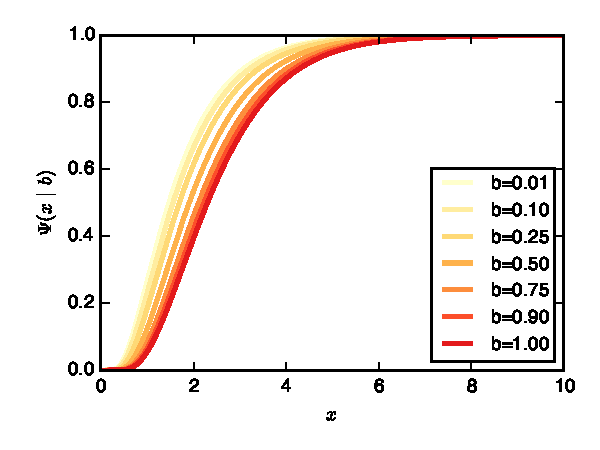
\includegraphics[width=\textwidth]{psi}
  \end{subfigure}
  \vspace{-2em}
  \caption{Plot of~$\Psi(x \given b)$, the conditional acceptance
    probability for a proposed value of~$x$, for~$b\in (0,1]$. In all
    cases, this function is monotonically increasing from 0 to 1 as a
    function of~$x$, and thus defines a cumulative distribution
    function. }
\label{fig:psi}
\end{figure}


The~$\distJacobi(x \given b)$ density can be written as an inverse 
gamma distribution times one minus a cumulative distribution function:
\begin{align}
  \distJacobi(x \given b) &= \frac{b 2^b}{\sqrt{2\pi x^3}} 
      \exp \left \{ -\frac{-b^2}{2x} \right \}
      \left[\sum_{n=0}^\infty (-1)^n \frac{\Gamma(n+b)}{b \Gamma(b) \Gamma(n+1)} (2n+b)
            \exp\left\{- \frac{4n^2 +4nb}{2x} \right\} \right]. \\
  &= 2^b \distInvGamma \left(x \given \tfrac{1}{2}, \tfrac{b^2}{2} \right) \left( 1 - \Psi(x \given b) \right),
\end{align}
where the inverse gamma distribution is
\begin{align}
  \distInvGamma(x \given \tfrac{1}{2}, \tfrac{b^2}{2})
  &= \frac{\sqrt{b^2/2}}{\Gamma(\tfrac{1}{2})} x^{-\tfrac{3}{2}} \exp\left\{-\frac{b^2}{2x} \right\} \\
  &= \frac{b}{\sqrt{2 \pi x^3}} \exp\left\{-\frac{b^2}{2x} \right\},
\end{align}
and where we have defined~$\Psi(x \given b)$ such that,
\begin{align}
1-\Psi(x \given b) &=
    \sum_{n=0}^\infty (-1)^n \frac{\Gamma(n+b)}{\Gamma(n+1)} \frac{2n+b}{\Gamma(b+1)}
    \exp\left\{- \frac{2n(n+b)}{x} \right\}  
\end{align}
Empirically, we have found that~$\Psi(x \given b) \in [0,1]$. Moreover,~$\Psi(x \given b)$ appears to be monotonically increasing, with~$\lim_{x \to 0} \Psi(x \given b) = 0$, and~$\lim_{x \to \infty} \Psi(x \given b) = 1$. In other words,~$\Psi(x \given b)$ defines a cumulative distribution function. Figure~\ref{fig:psi} plots this function for various values of~$b$. 

Since~$\Psi(x \given b)$ is a
CDF,~$2^b \distInvGamma(x \given \tfrac{1}{2}, \tfrac{b^2}{2})$
dominates~$\distJacobi(x \given b)$, making the inverse gamma a
natural proposal distribution.  The acceptance probability~$2^{-b}$,
which decreases from~$1$ to~$\tfrac{1}{2}$ as~$b$ goes from~$0$
to~$1$. In the worst case, when~$b=1$, rejection sampling with an
inverse gamma proposal will take~$2$ proposals on average.

To determine whether a proposed value of~$x$ is accepted, we must
sample~$u \sim \mathrm{Unif}(0,1)$, and check
whether~$u < 1-\Psi(x \given b)$. This is sometimes referred to as
``generalized'' rejection sampling~\cite{devroye1986}.
We have found that the infinite sum
in the definition of~$\Psi(x \given b)$ converges in a small number of
terms, and can be reasonably approximated as discussed below. 
%In practice, we truncate it at ten terms.

It would be particularly nice if~$1-\Psi(x \given b)$ corresponded to
a cumulative distribution function of a known distribution that we can
efficiently sample from. If so, we would not have to evaluate the
infinite sum. Unfortunately, we have not been able to equate this to a
well-known distribution function.

\subsection{Rejection sampling~$\distJacobi(x \given b,z)$}

\begin{figure}
\centering
  \begin{subfigure}[t]{4in}
    \centering
    \vskip 0pt
    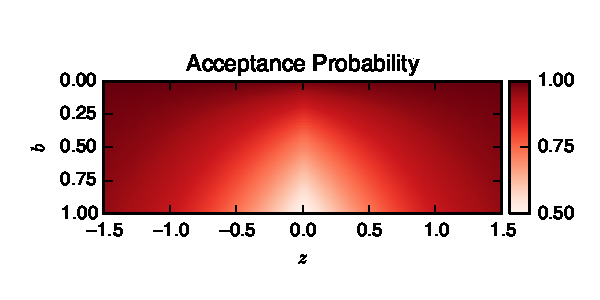
\includegraphics[width=\textwidth]{acceptance}
  \end{subfigure}
  \vspace{-2em}
  \caption{Acceptance probability as a function of~$b$ and~$z$.}
\label{fig:acceptance}
\end{figure}

We can do the same for the tilted Jacobi density,~$\distJacobi(x \given b,z)$.
\begin{align}
  \distJacobi(x \given b, z) 
  &= \cosh^b(z) \frac{b 2^b}{\sqrt{2\pi x^3}} 
    \exp \left \{ -\frac{-b^2}{2x} - \frac{xz^2}{2} \right \}
    \left( 1-\Psi(x \given b) \right) \\
  &= \cosh^b(z) \frac{b 2^b}{\sqrt{2\pi x^3}} 
    \exp \left \{ -\frac{z^2}{2x} \left[\left( \frac{b}{z} \right)^2 + x^2 \right]\right \}
    \left( 1-\Psi(x \given b) \right) \\
  &= \cosh^b(z) \frac{b 2^b}{\sqrt{2\pi x^3}} 
    \exp \left \{ -\frac{z^2}{2x} \left[\left( x- \frac{b}{|z|} \right)^2  +\frac{2bx}{|z|}\right]\right \}
    \left( 1-\Psi(x \given b) \right) \\
  %&= \cosh^b(z) \frac{b 2^b}{\sqrt{2\pi x^3}} 
  %  \exp \left \{ -\frac{\left(\tfrac{|z|}{b}\right)^2 b^2}{2x} \left( x- \frac{b}{|z|} \right)^2  
  %  -b|z| \right \} 
  %  \left( 1-\Psi(x \given b) \right) \\
  &= 2^b \, \cosh^b(z) \, e^{-b|z|} \,
    \distInvGaussian \left(x \, \bigg| \, \frac{b}{|z|}, \, b^2 \right) 
    \left( 1-\Psi(x \given b) \right),
\end{align}
where~$\distInvGaussian(\cdot)$ denotes the inverse Gaussian density,
\begin{align}
\distInvGaussian\left(x \, \bigg| \, \frac{b}{|z|}, \, b^2 \right) 
  &= \left( \frac{b^2}{2\pi x^3} \right)^{1/2} 
    \exp \left \{ - \frac{b^2 \left(x - \tfrac{b}{|z|} \right)^2}{2 \left(\tfrac{b}{|z|} \right)^2 x}   \right \} \\
  &= \frac{b}{\sqrt{2\pi x^3}}
    \exp \left \{ - \frac{z^2}{2x}  \left(x - \frac{b}{|z|} \right)^2   \right \}.
\end{align}

The scaling constant simplifies to,
\begin{align}
2^b \, \cosh^b(z) \, e^{-b|z|} 
  &= 2^b \cosh^b(|z|) \, e^{-b|z|} \\
  &= 2^b \left(\frac{(1+e^{-2|z|}) e^{-|z|}}{2e^{-|z|}} \right)^b \\
  &= \left(1 + e^{-2|z|} \right)^b.
\end{align}
When~$z=0$, this equals~$2^b$, the same scaling constant as above. When~$|z|>0$, the scaling constant is still greater than one, as required for rejection sampling, but it is even less than~$2^b$, making an even better proposal distribution. Figure~\ref{fig:acceptance} plots the acceptance probability as a function of~$b$ and~$z$.


\subsection{Approximating the conditional acceptance threshold}
Let,
\begin{align}
1-\Psi(x \given b) 
  &=
    \sum_{n=0}^\infty (-1)^n \frac{\Gamma(n+b)}{\Gamma(n+1)} \frac{2n+b}{\Gamma(b+1)}
    \exp\left\{- \frac{2n(n+b)}{x} \right\} \\
  &= \sum_{n=0}^\infty (-1)^n \psi_n(x \given b).
\end{align}
We have,
\begin{align}
\psi_0(x \given b) &= 1 \\
\psi_1(x \given b) &= (2+b) e^{-2(b+1) / x} \\
\psi_2(x \given b) &= \frac{(1+b)(4+b)}{2} e^{-4(b+2) / x} \\
\psi_3(x \given b) &= \frac{(2+b)(1+b)(6+b)}{6} e^{-6(b+3) / x} \\
\nonumber \ldots & \\
\psi_n(x \given b) &= \frac{\left(\prod_{j=1}^{n-1} (j+b) \right) (2n+b)}{n!} e^{-2n(n+b)/x} 
  % \\
  %                  &= \frac{\left((n-1)! + \frac{n(n-1)}{2} b + o(b^2) \right) (2n+b)}{n!} e^{-2n(n+b)/x} \\
  % &= \left( 2 + \left(\frac{n}{(n-2)!} + \frac{1}{n} \right)b + o(b^2) \right) e^{-2n(n+b)/x}.
  % &= \left( \frac{1}{n} + \frac{b}{2(n-2)!} + o(b^2) \right) (2n+b) e^{-2n(n+b)/x}.
\end{align}
Higher order terms rapidly diminish extremely quickly due to the
exponential term. In practice, the first six terms are enough to
approximate~$1-\Psi(x \given b)$ with satisfactory precision. 
% Thus, we have,
% \begin{align}
% 1-\Psi(x \given b) 
%   &\approx 1 - (2+b) e^{-2(b+1) / x} + \frac{(1+b)(4+b)}{2} e^{-4(b+2) / x} - \frac{(2+b)(1+b)(6+b)}{6} e^{-6(b+3) / x}.
% \end{align}

\section{Discussion}
We have derived a rejection sampling algorithm for the \polyagamma distribution 
in the small shape parameter regime, i.e. where~$b \in (0,1]$. This is 
particularly relevant to Bayesian marginal likelihood calculations with 
annealed importance sampling, as well as to the simulation of L\'{e}vy 
processes with \polyagamma increments. Our approach is based on the observation 
that the Jacobi density factorizes into the product of a scaling coefficient, 
an inverse Gaussian density, and one minus a cumulative distribution function.
The scaling coefficient is~$2^b$, which implies that the acceptance probability 
is uniformly bounded below at~$0.5$, and exponentially increases toward one 
as~$b$ goes to zero. 

\bibliography{draft}
\bibliographystyle{unsrtnat}


\end{document} 

